\documentclass[xcolor=dvipsnames]{beamer}
\usepackage{lmodern}
\usepackage[most]{tcolorbox}
\tcbset{beamer,colback=blue!20!white,colframe=blue!75!black}
\usepackage[absolute,overlay]{textpos}
\usepackage{graphicx}

\usetheme{Antibes}

\title[Version Control Systems for PyQFP]{Version Control System Suggestion for PyQFP}
\subtitle[Karl Everst]{Git, Git workflows and GitHub}
\author[Karl Everst]{Karl Everst}

\begin{document}

\AtBeginSection[]
{
	\begin{frame}
		\frametitle{Outline}
		\tableofcontents[currentsection]
	\end{frame}
}

\AtBeginSubsection[]
{
	\begin{frame}
		\frametitle{Outline}
		\tableofcontents[currentsubsection]
	\end{frame}
}

\begin{frame}
\titlepage
\end{frame}

\begin{frame}
\frametitle{Outline}
\tableofcontents[]
\end{frame}

\section{Introduction to VCS}

\begin{frame}{What is a Version Control System (VCS)?}

\begin{itemize}

	\item System that records changes to a file or set of files.
	\item Classically local VCSs had a simple database system.
	\item To collaborate with other developers centralized VCS (CVCS) were created.
	\\Advantage: Everyone is on the same page.
	\\Donwside: Single Point of failure.
	\item Next step of the VCS evolution are the distributed VCS (DVCS) such as GIT and
	Mercurial amongst others.

\end{itemize}

\end{frame}

\begin{frame}{You want from this...}

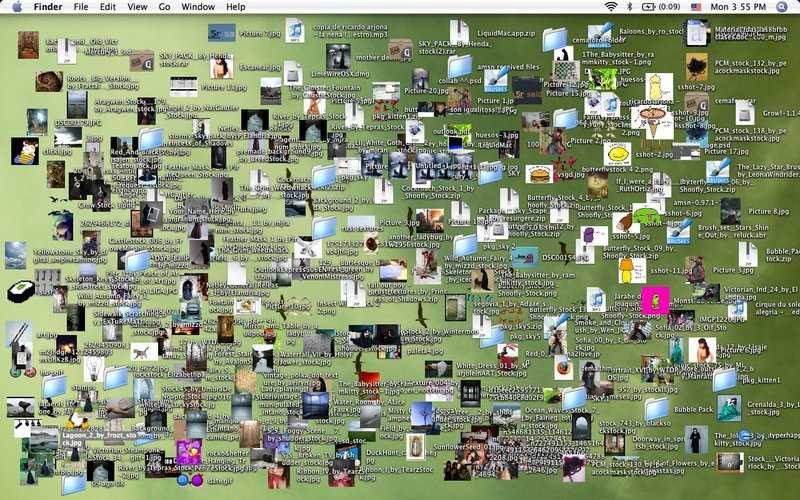
\includegraphics[width = 0.9\textwidth]{messy.jpg}

\end{frame}

\begin{frame}{...to this.}


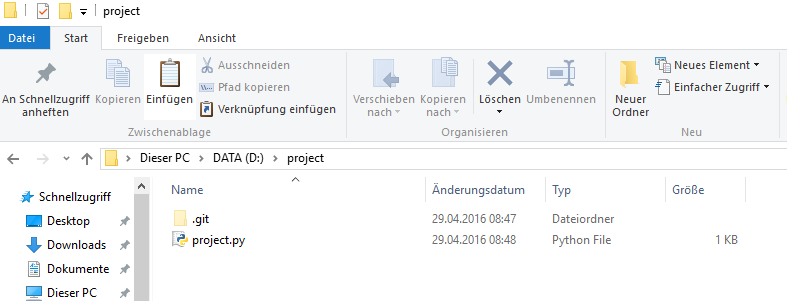
\includegraphics[width = 0.8\textwidth]{ordentlich.png}
\\
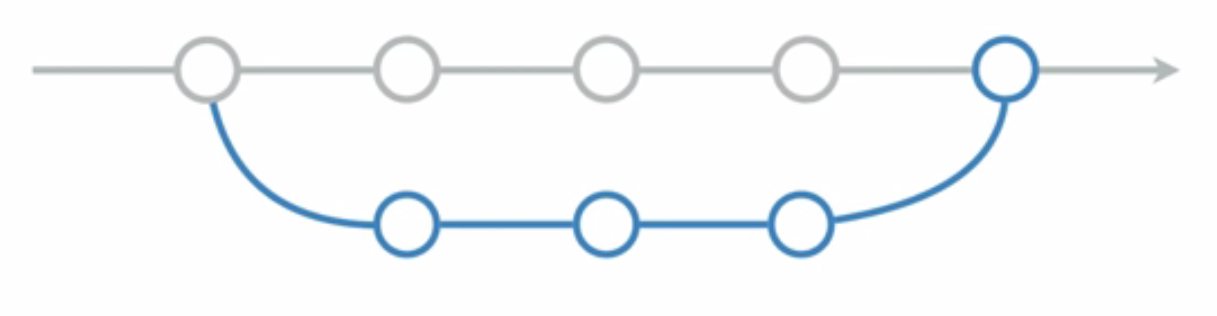
\includegraphics[width = 0.8\textwidth]{ordentlich2.png}


\end{frame}


\section{Git}

\subsection{History}

\begin{frame}{Introduction to Git}

\begin{textblock*}{12cm}(0.5cm,2.5cm) % {block width} (coords)
\begin{itemize}

	\item In 2002, the Linux kernel project began using proprietary DVCS called BitKeeper.
	\item In 2005, BitKeeper went commercial so that the Linux community had to develop 				own DVCS. This prompted Linus Torvalds to create Git.
	\item Strenghts of Git are speed, efficiency and the branching system for nonlinear
	      development.

\end{itemize}
\end{textblock*}

\begin{textblock*}{5cm}(0.5cm,6.5cm) % {block width} (coords)
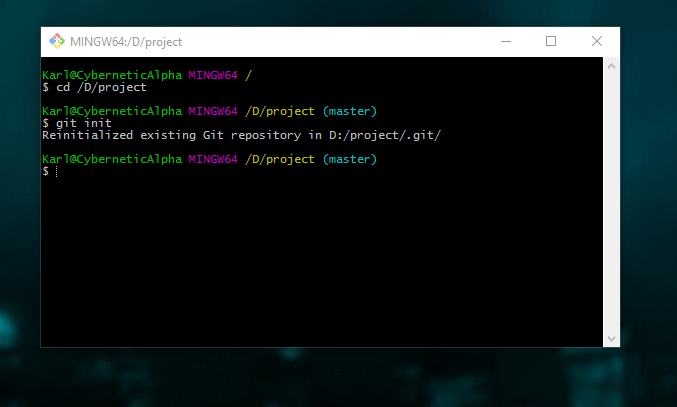
\includegraphics[width = 0.9\textwidth]{gitConsole.png}
\end{textblock*}

\end{frame}

\subsection{Commands}

\begin{frame}{Git Commands}

\begin{tcolorbox}[title=git clone]
Makes a Git repository copy from a remote source.
\end{tcolorbox}

\begin{tcolorbox}[title=git commit]
Takes all of the changes written in the index, creates a new commit object pointing to it and sets the branch to point to that new commit.
\end{tcolorbox}

\end{frame}

\begin{frame}{Git Commands}

\begin{tcolorbox}[title=git branch]
Creates a new branch if a branch name is provided.
\end{tcolorbox}

\begin{tcolorbox}[title=git merge]
Merges one or more branches into your current branch and automatically creates a new commit if there are no conflicts.
\end{tcolorbox}

\end{frame}

\begin{frame}{Git Commands}

\begin{tcolorbox}[title=git pull]
Fetches the files from the remote repository and merges it with your local one.
\end{tcolorbox}

\begin{tcolorbox}[title=git push]
Pushes all the modified local objects to the remote repository and advances its branches.
\end{tcolorbox}

\end{frame}

\subsection{Workflows}

\begin{frame}{Git Workflows - Linear Development}

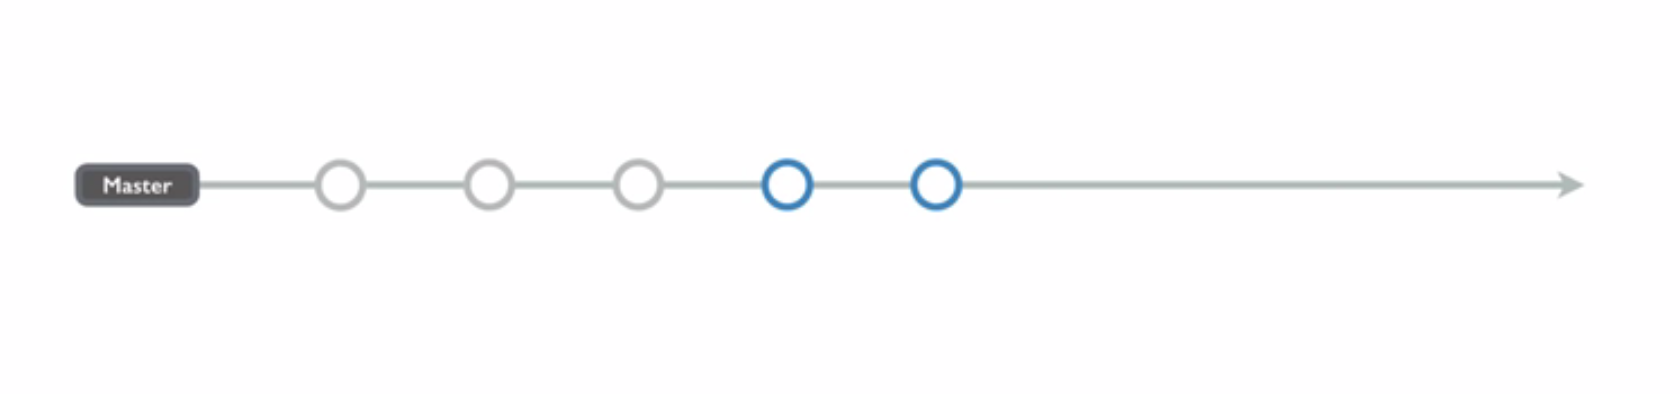
\includegraphics[width = 0.8\textwidth]{linearDevelopment.png}

\end{frame}

\begin{frame}{Git Workflows - Nonlinear Development - Branching}

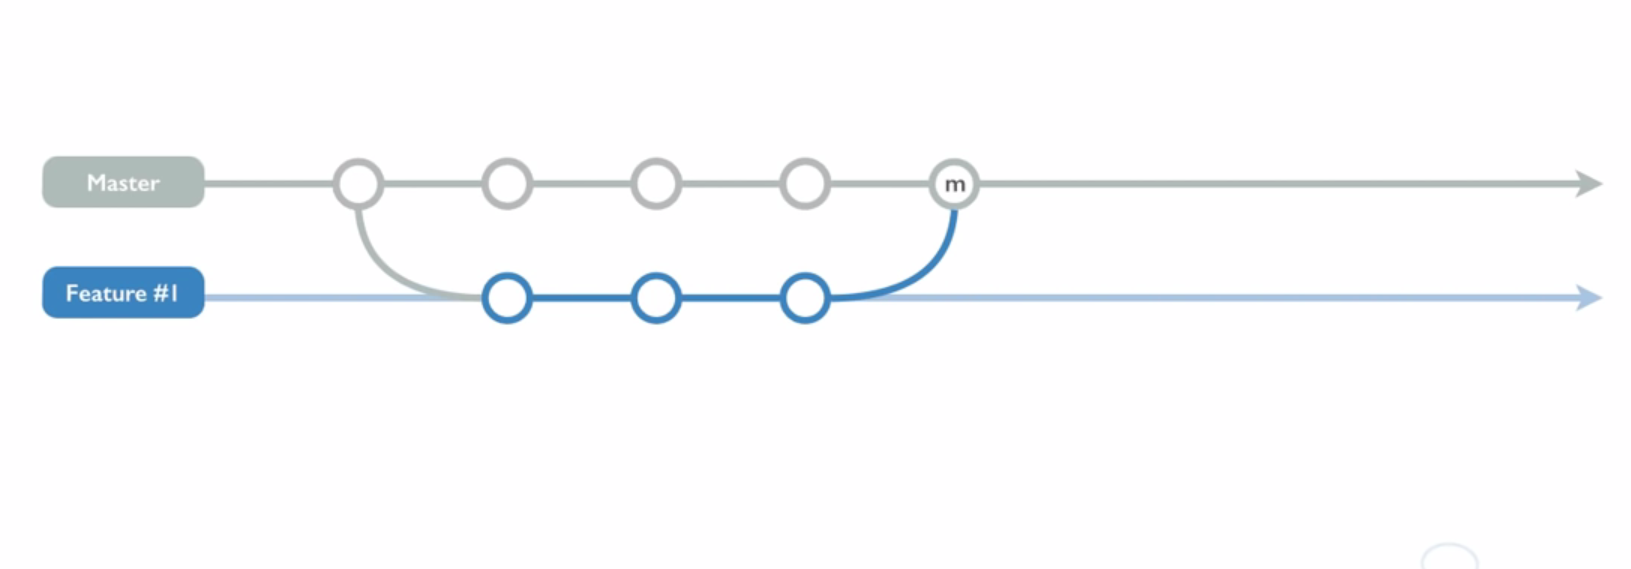
\includegraphics[width = 0.8\textwidth]{nonlinearDevelopment.png}

\end{frame}

\begin{frame}{Git Workflows - More Sophisticated Techniques}

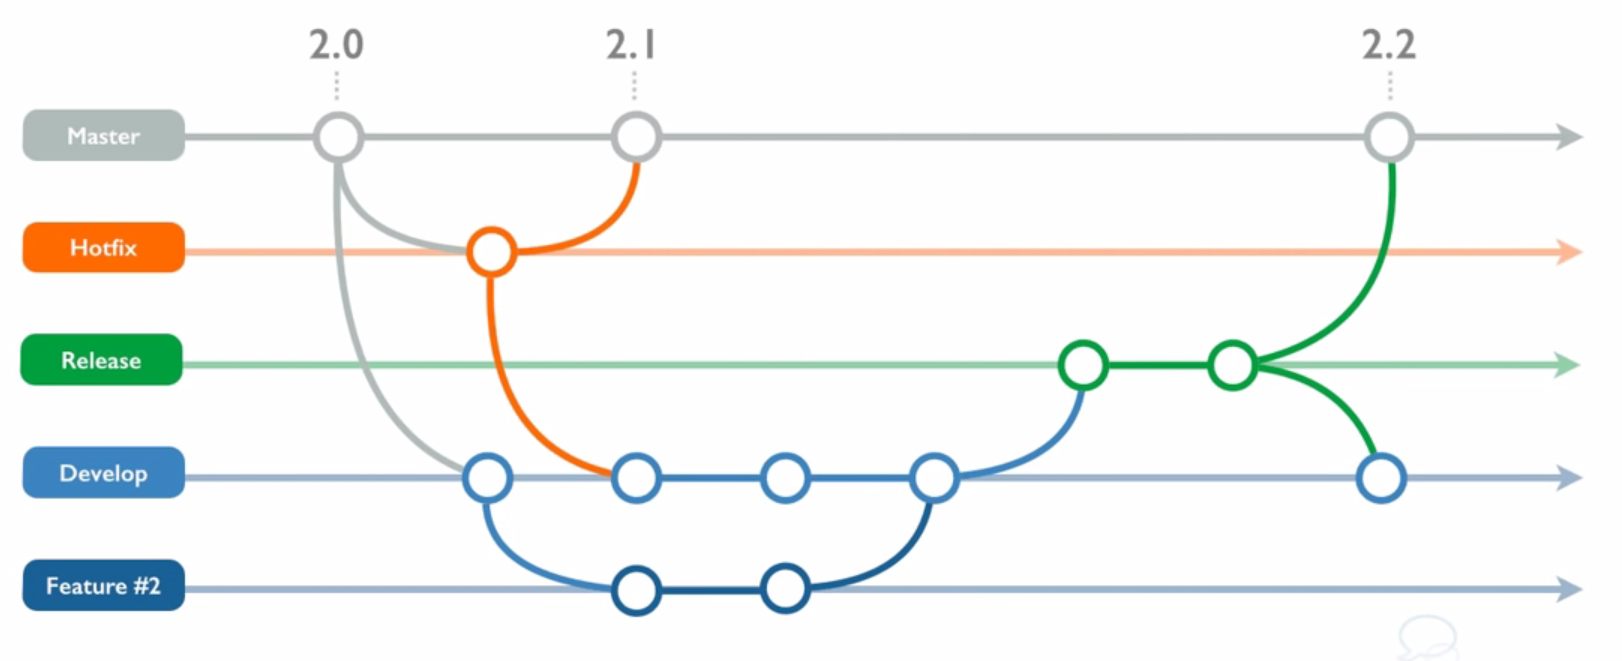
\includegraphics[width = 0.8\textwidth]{sophisticatedTechniques.png}

\end{frame}

\section{Online Repositories}

\subsection{BitBucket}

\begin{frame}{BitBucket Keynotes}

\begin{itemize}

	\item Bitbucket is an online repository service for projects that use either the Mercurial or Git as DVCS.
	\item URL: https://bitbucket.org/
	\item Up to 5 users can use BitBucket for free creating infinite amount of repositories which can also be private.
\\~\\For comparison: GitHub provides no private repositories for free users.

\end{itemize}

\end{frame}

\begin{frame}{Using BitBucket}

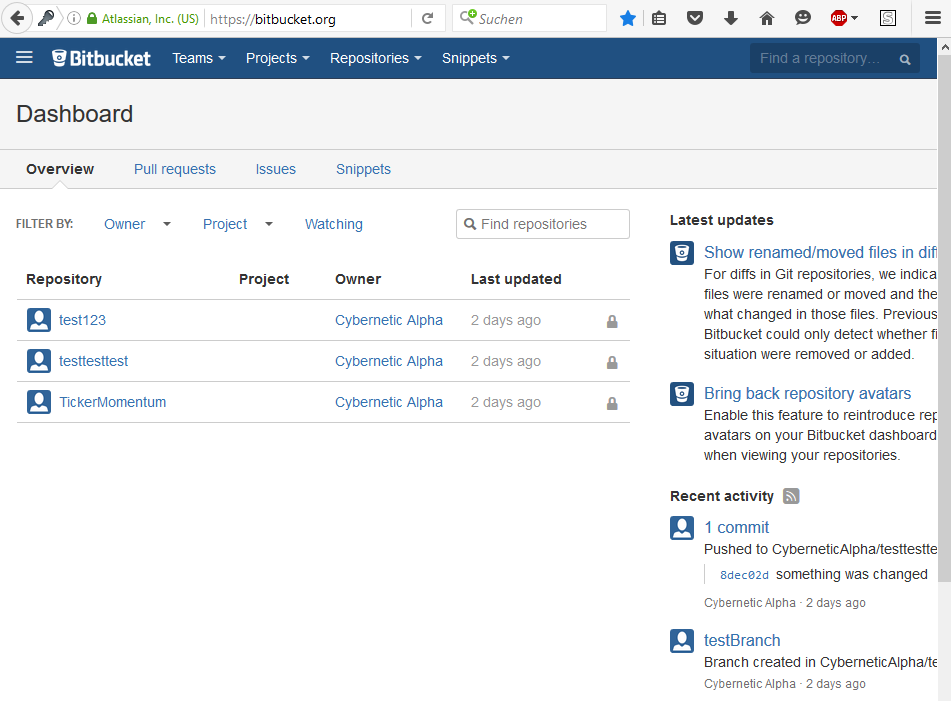
\includegraphics[width = 0.8\textwidth]{bitBucket.png}

\end{frame}

\subsection{GitHub}

\begin{frame}{GitHub Keynotes}

\begin{itemize}

	\item GitHub is an online repository service for projects that use Git as DVCS.
	\item URL: https://github.com/
	\item GitHub can be used for free for public repositories.

\end{itemize}

\end{frame}

\begin{frame}{Using GitHub}

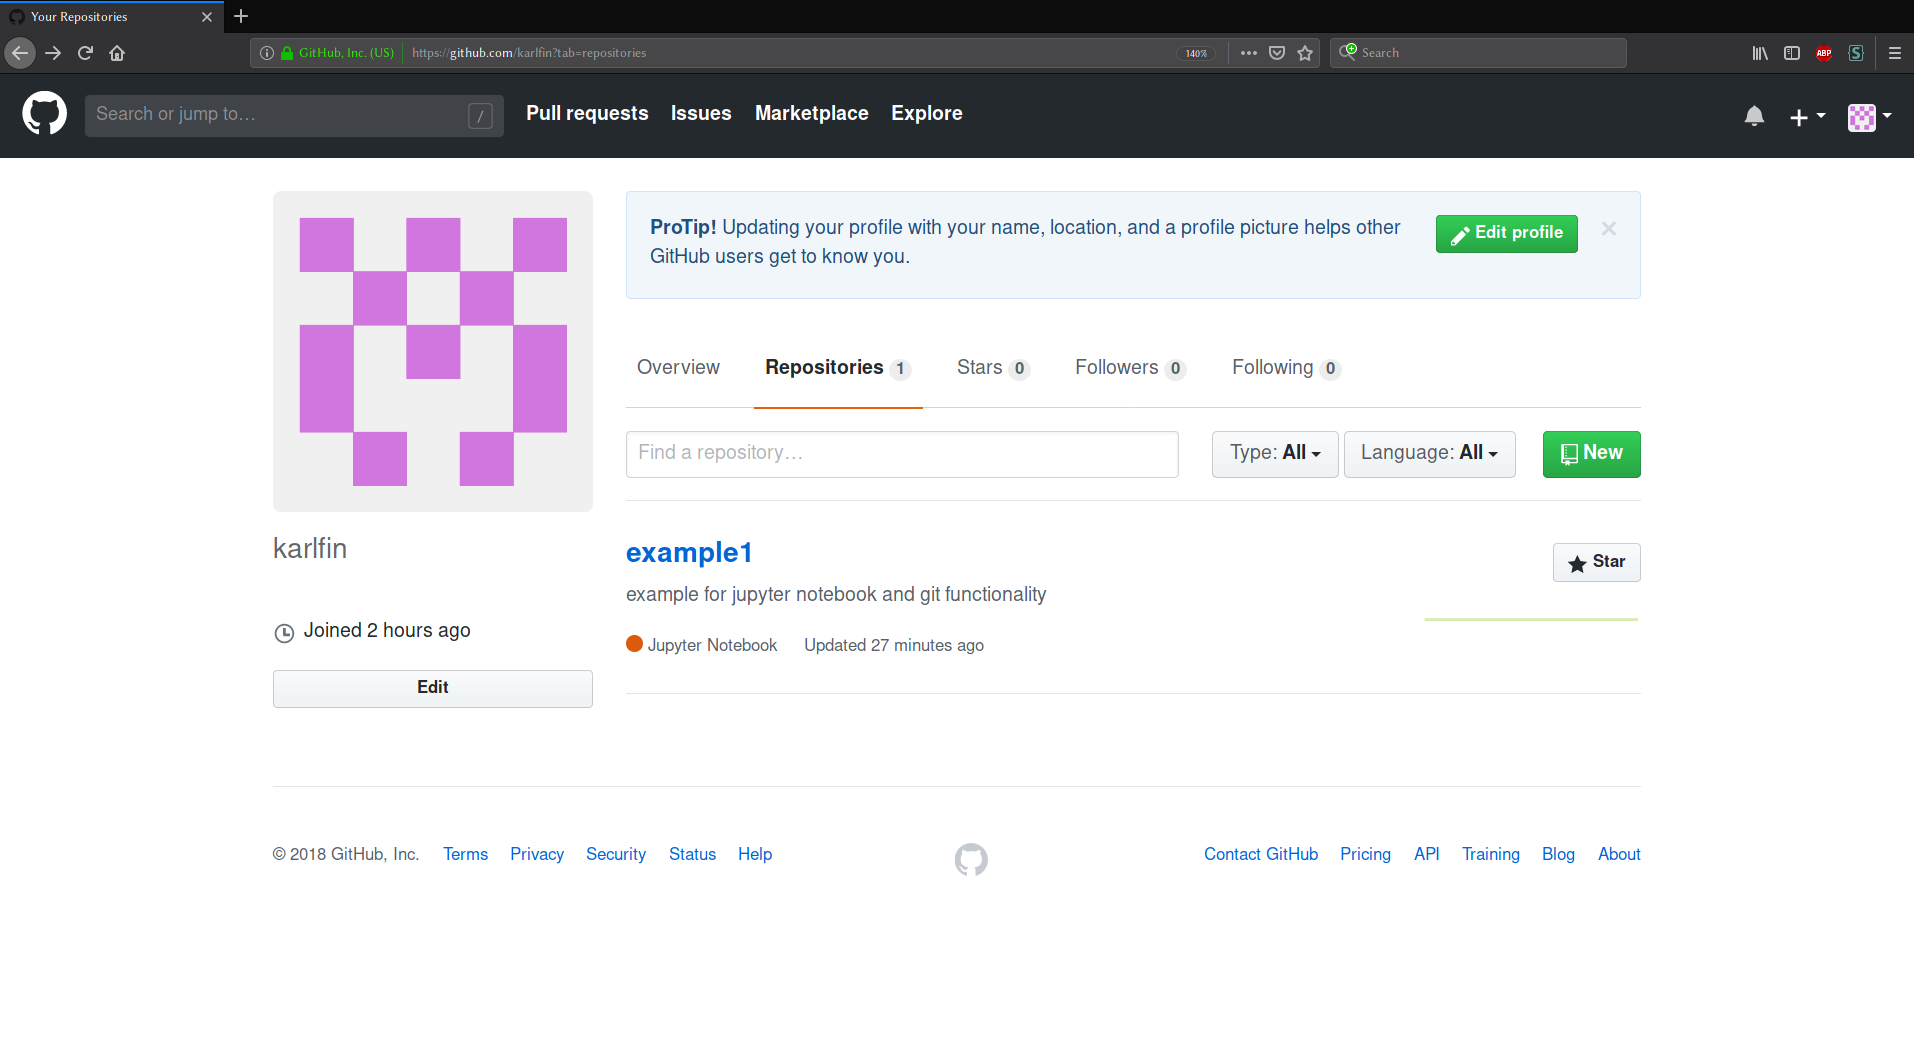
\includegraphics[width = 0.8\textwidth]{github.png}

\end{frame}

\section{GUI-Client for Git: GitKraken}

\begin{frame}{GitKraken Keynotes}
\begin{itemize}

	\item A free Git client for Windows, Mac and Linux.
	\item URL: https://www.gitkraken.com/
	\item Takes over Git console usage which adds to user friendliness.

\end{itemize}
\end{frame}

\begin{frame}{Using GitKraken}

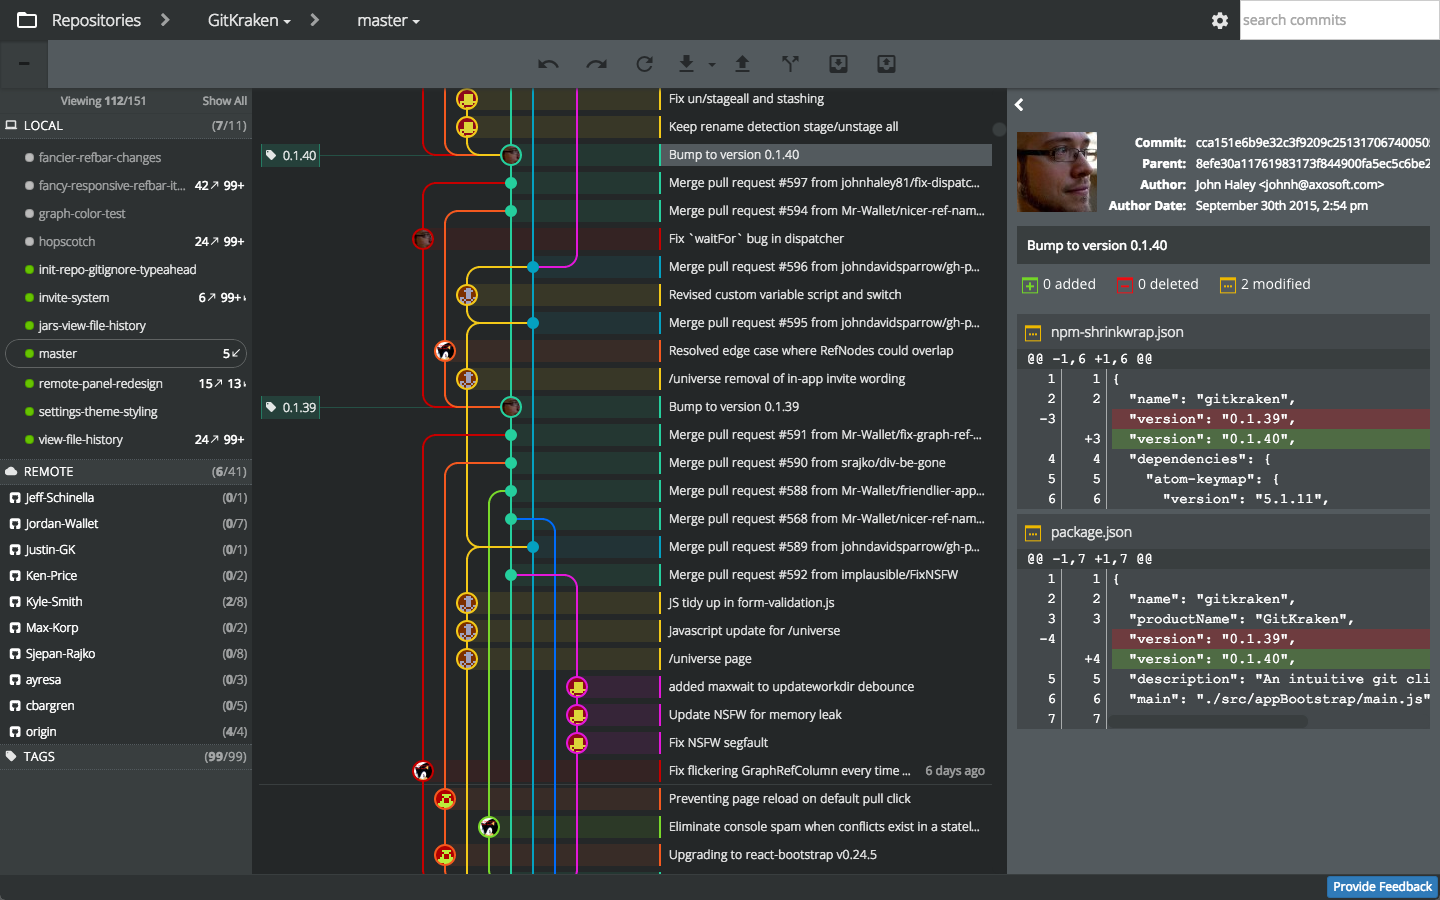
\includegraphics[width = 0.8\textwidth]{gitkraken.png}

\end{frame}

\section{}

\begin{frame}{The End}

%\centering \Large
%Thank you for your attention!
%\emph{Fin}
\begin{textblock*}{10cm}(2cm,3.5cm) % {block width} (coords)

\includegraphics[width = 0.8\textwidth]{thankYou.png}
\end{textblock*}

\end{frame}

\end{document}
